\begin{figure*}
    \centering
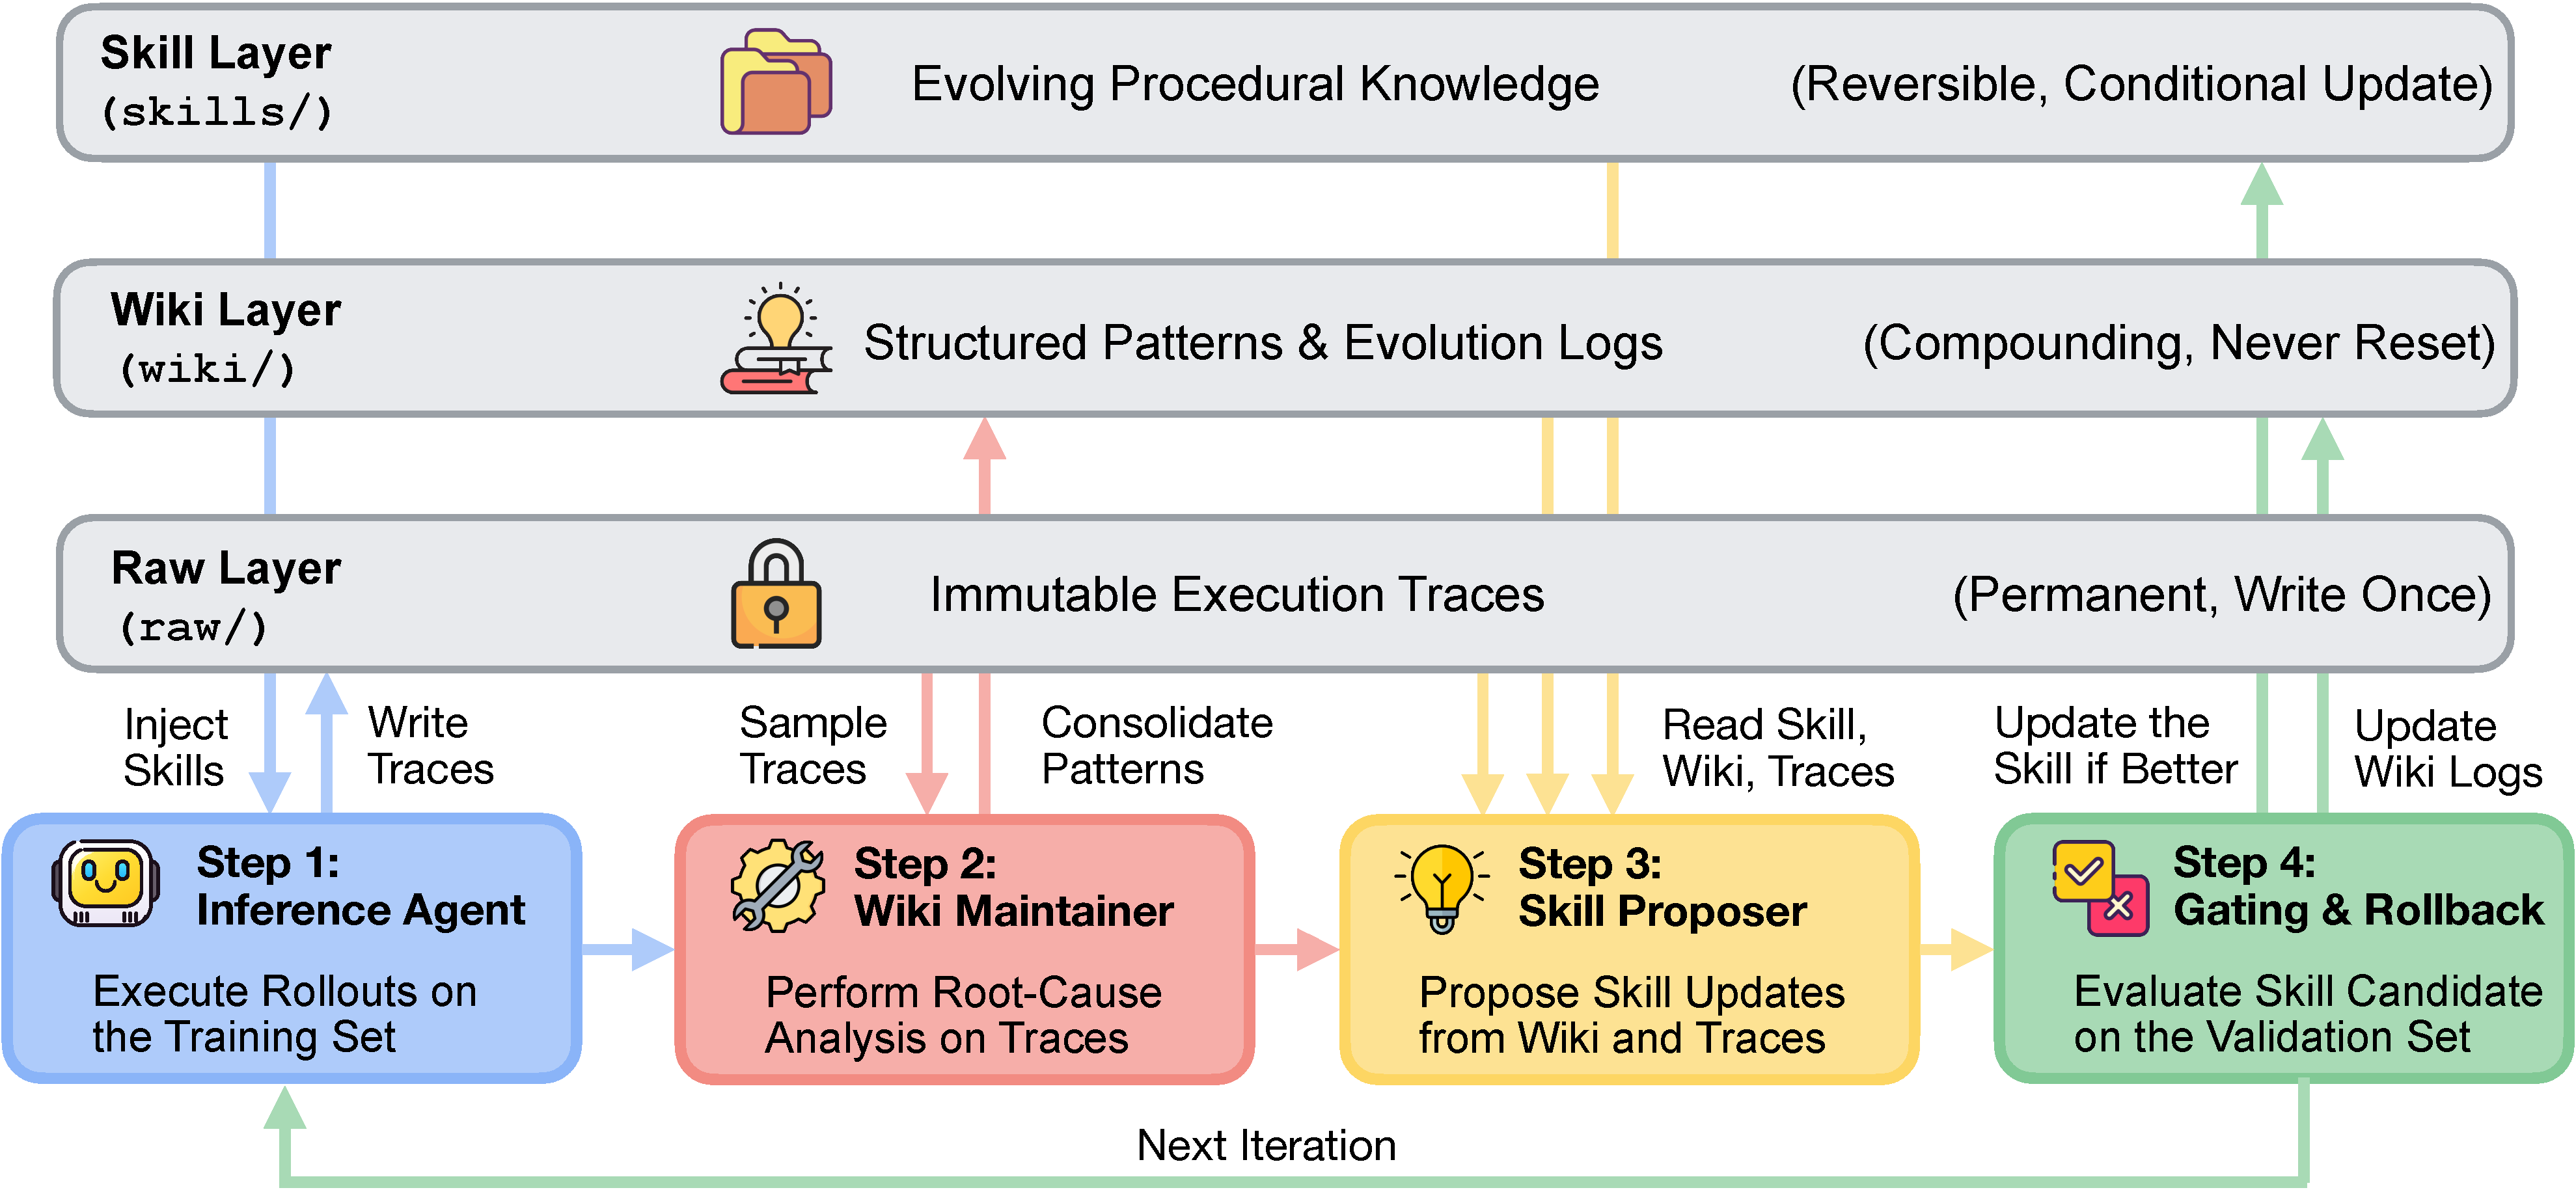
\includegraphics[width=\textwidth]{figures/wikiskill-diagram.pdf}
\caption{\textbf{Overview of the WikiSkill framework.} The agent workspace is structured into three layers: immutable execution traces (Raw Layer), a persistent knowledge base that compounds across iterations (Wiki Layer), and active procedural instructions (Skills Layer). In each evolutionary loop, the Inference Agent runs rollouts (injecting active skills but restricting Wiki access), the Wiki Maintainer consolidates traces into the Wiki, and the Skill Proposer (with the ReAct mechanism) suggests updates while the Wiki is retained across all iterations.}
\label{figure:wikiskill_diagram}
\end{figure*}
